%# -*- coding: utf-8-unix -*-
%%==================================================
\chapter{RocketMq}
\label{chap1}
\begin{itemize}[noitemsep,topsep=0pt,parsep=0pt,partopsep=0pt]
	\item ...
\end{itemize}

\section{知识点和方法论}

\subsection{知识点}
NameServer:主要负责对于源数据的管理,包括了对于Topic和路由信息的管理。

每个 Broker 在启动的时候会到 NameServer 注册,
Producer 在发送消息前会根据 Topic 到 NameServer 获取到 Broker 的路由信息,Consumer 也会定时获取 Topic 的路由信息。


\subsubsection{信息流}
生产阶段,Producer 新建消息,然后通过网络将消息投递给 MQ Broker
存储阶段,消息将会存储在 Broker 端磁盘中
消息阶段, Consumer 将会从 Broker 拉取消息

生产阶段

生产者(Producer) 通过网络发送消息给 Broker,当 Broker 收到之后,将会返回确认响应信息给 Producer。所以生产者只要接收到返回的确认响应,就代表消息在生产阶段未丢失。

消费者有两种消费模式, 一种是DefaultMQPushConsumer和DefaultMQPullConsumer模式, 一是推送消息, 一个是拉取消息.

push: consumer向broker发出请求, 保持了一种长连接, broker会每5s检测一次是否有消息, 如果有消息, 则将消息推送给consumer. 使用DefaultMQPushConsumer实现消息消费, broker会主动记录消息消费的偏移量

pull: 是消费方主动去broker拉取诗句, 一般会在本地使用定时任务实现, 使用它获得消息状态方便, 负载均衡心梗可控, 但消息的及时性差, 而且需要手动记录消息消费的偏移量, 所以在工作中多数情况推荐使用Push模式.



\begin{figure}
	\centering
	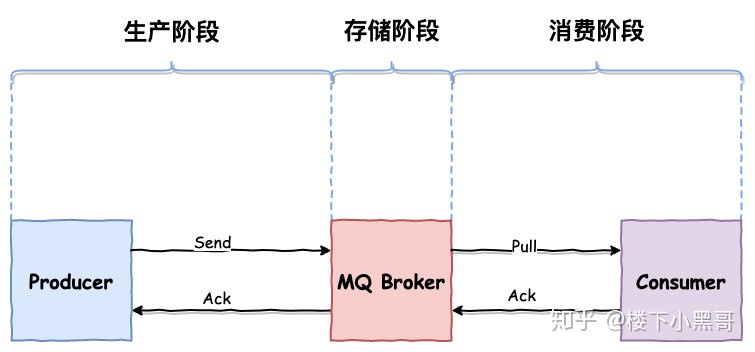
\includegraphics[width=0.7\linewidth]{figures/rocketmqlife.jpg}
	\caption{rocketmqlife}
	\label{fig:rocketmqlife}
\end{figure}


Broker 存储阶段

将会优先保存到内存中,然后立刻返回确认响应给生产者。随后 Broker 定期批量的将一组消息从内存异步刷入磁盘。

\subsubsection{消息队列如何保证消息可靠传输}

1. 保证消息不重复. 生产者不能重复生产消息

2. 消息不能少, 消息不丢失, 生产者发送的消息, 消费者一定要能消费到, 对于这个问题

a. 生产者发送消息时, 要确认broker确实收到并持久化了这条消息. ack机制.
b. broker要等待消费者真正确认消费到了消息时才删除掉消息, 通过消费端的ack机制.

消息实现的时候, 需要一定的幂等性操作. 如果有两条重复的消息发送过来了, 在数据库层面需要做好操作比如插入订单号, 如果已经有了就把这个订单号丢弃.

\subsubsection{消息队列有哪些作用}

1. 解耦: 两个系统的直接通讯方式, 两个系统不需要相互依赖

2. 异步: 系统A给消费队列发送完消息之后, 就可以继续做其他事情了

3. 流量削峰: 如果使用消息队列的方式来调用某个系统, 那么消息将在队列中排队, 由消费者自己控制消费速度.

\subsubsection{RocketMQ架构设计}
nameserver: 独立, 不进行通信, 维护路由信息, 存储了发送者是谁, 消费者是谁, broker是谁


broker: 和每一个nameserver建立一个长连接.

-- topic:

---- queue: 和消费者负载均衡

producer: 拉取topic所属的broker,

CommitLog: 消息内容, 不区分topic

ConsumeQueue: 基于topic的索引文件

IndexFile: 通过key或时间区间.
\subsubsection{RocketMQ事物型消息}
依赖TransactionListener接口

executeLocalTransaction 方法会在发送消息后调用, 用于执行本地事物, 如果本地事物执行成功, rocketmq再提交消息.

简单来说, 两阶段提交, 消息先提交到RMS\_SYS\_TRANS\_HALF\_TOPIC的topic中, 而不是投递到真正的topic中. 当commit成功之后, 将消息投递到真实的topic中, 然后把先提交的地方删除, 如果是rollback只把第一次提交到的地方删除.
